% !TEX TS-program = pdflatex
% !TeX program = pdflatex
% !TEX encoding = UTF-8
% !TeX spellcheck = en_US

\documentclass[11pt, a4paper]{article}
%\usepackage{fullpage}
\usepackage[left=1cm,right=1cm,top=1cm,bottom=2cm]{geometry}
\usepackage[fleqn]{amsmath}
\usepackage{amssymb}
%\usepackage{indentfirst}
\usepackage[T1]{fontenc}
\usepackage[utf8]{inputenc}
\usepackage[french,english]{babel}
\usepackage{txfonts} 
\usepackage[]{graphicx}
\usepackage{multirow}
\usepackage{hyperref}
\usepackage{parskip}
\usepackage{multicol}
\usepackage{wrapfig}

\usepackage{turnstile}%Induction symbole

\usepackage{tikz}
\usetikzlibrary{arrows, automata}
\usetikzlibrary{decorations.pathmorphing}

\renewcommand{\baselinestretch}{1}

\setlength{\parindent}{24pt}


\begin{document}

%\selectlanguage {french}
%\pagestyle{empty} 

\noindent
\begin{tabular}{ll}
	\multirow{3}{*}{
\includegraphics[width=1.5cm]{../../extra/logo/esi.ml.pdf}} & \'Ecole national Supérieure d'Informatique, Algiers, Algeria\\
	& 2CSSIL2/2CSSIQ2 (2023/2024)\\
	& Machine Learning (ML)
\end{tabular}\\[.25cm]
\noindent\rule{\textwidth}{1pt}\\[-0.5cm]
\begin{center}
	{\LARGE \textbf{Workshop 03: Advanced neural networks}}
	\begin{flushright}
		Dr. Abdelkrime Aries
	\end{flushright}
\end{center}\vspace{-.25cm}
\noindent\rule{\textwidth}{1pt}

\section*{Information}

\begin{itemize}
	\item \textbf{APIs}: tensorflow, scikit-learn, numpy, jupyter notebook, pandas, matplotlib
	\item \textbf{Datasets}: Pokemon Image Dataset : {\scriptsize\url{https://www.kaggle.com/datasets/vishalsubbiah/pokemon-images-and-types}}
	\item \textbf{Documentation}: Demo ({\scriptsize \url{https://github.com/projeduc/ESI_ML/tree/main/demos/NN}}), Tensorflow ({\scriptsize \url{https://www.tensorflow.org/api_docs/python/tf/}})
	\item \textbf{Pre-processing}: Provided with this workshop (you must rename the dataset folder as "pokemon" or change the path of the dataset in the provided code)
\end{itemize}

\section{Clustering}

In this section, we will try implementing auto-encoders to cluster Pokemons. 
To do this, we will define an abstract class \textbf{ClusterA} which has two implementations as shown in figure \ref{fig:pok-cluster-CD-en}.
%We suppose, a perfect clustering is the one grouping similar types of Pokemons together.
Here is the description of some methods: 
\begin{itemize}
	\item \textbf{\_\_init\_\_}: Takes code size and input shape \textbf{in\_shape} as parameters.
	It defines the encoder and decoder layers in figure \ref{fig:CNN-pok-cls}.
	For \textbf{model.summary()} to work, we need to create the graph. So add this code after defining layers:
	\begin{verbatim}
		inimg = Input(shape=in_shape)
		super().__init__(inimg, self.call(inimg))
	\end{verbatim}
	\item \textbf{encode}: Takes an image as input and generates a code.
	\item \textbf{decode}: Takes a code as input and generates an image.
	\item \textbf{call}: Overrides a method of the super-class. 
	This method is used to call the object of this class as if it was a function.
	In our case, it is a whole encoder-decoder; it takes an image and generates a reconstruction of this image.
	\item \textbf{train\_step}: Takes a batch of images, applies a forward propagation followed by a backward one.
	\begin{verbatim}
		def train_step(self, data):
		with tf.GradientTape() as tape:
		img_pred = self.call(data)
		loss = self.loss(data, img_pred)
		
		variables = self.trainable_variables 
		gradients = tape.gradient(loss, variables)
		self.optimizer.apply_gradients(zip(gradients, variables))
		
		return {'loss': loss}
	\end{verbatim}
\end{itemize}

\begin{figure}[htp]
	\centering
	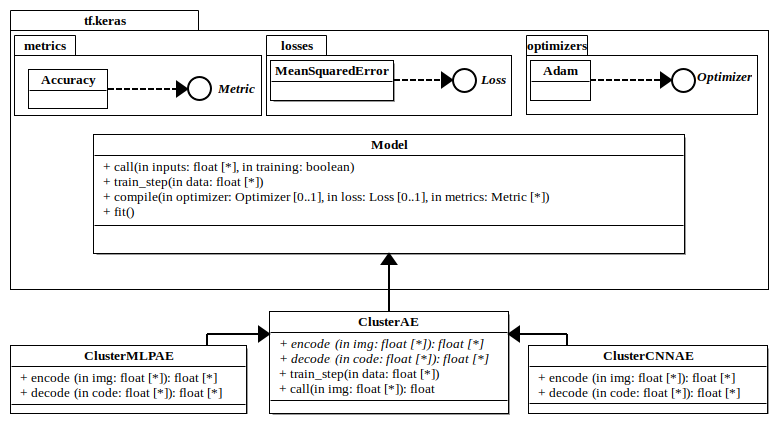
\includegraphics[width=0.6\textwidth]{../../img/workshop/pok-cluster-classD-en.png}
	\caption{Class diagrams of the two auto-encoders.}
	\label{fig:pok-cluster-CD-en}
\end{figure}

\subsection{MLP-based auto-encoder}

\begin{itemize}
	\item Design the model shown in figure \ref{fig:MLP-pok-cluster-en}.
	\item Create an auto-encoder model with a code of 2 (output of the encoder). 
	Compile the model and train it with Adam as optimizer and MSE as cost function.
	\item Generate training Pokemon codes.
	\item Plot their positions based on this code, indicating their types (color).
	\item Apparently a vector of 2 is not sufficient to represent the differences. 
	So, try training another model with a code of 10 elements. Generate training codes to be used for clustering.
	\item Apply K-Means on training Pokemon based on their codes. 
	Here, K is the number of classes.
	\item For each generated cluster, we assume that the majority class is the one represented by this cluster.
	\item Calculate Rand index: \textbf{sklearn.metrics.rand\_score}
%	\item Repeat the same with the CNN auto-encoder.
\end{itemize}

\begin{figure}[htp]
	\centering
	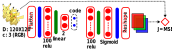
\includegraphics[width=0.6\textwidth]{../../img/workshop/MLP-pok-cluster-en.pdf}
	\caption{Architecture of MLP-based Pokemons' clustering Auto-encoder.}
	\label{fig:MLP-pok-cluster-en}
\end{figure}

\subsection{CNN-based auto-encoder}

\begin{itemize}
%	\item Design the model shown in figure \ref{fig:MLP-pok-cluster}.
	\item Design a CNN-based model. 
	You can inspire from the demo TF\_CNN part III.
	\item Repeat the same with the CNN auto-encoder.
\end{itemize}

\section{Classification}

In this section, we will try implementing some models for Pokemon classification.

\subsection{CNN-based classifier}

\begin{itemize}
	\item Design a model that classifies pokemons according to their types (see figure \ref{fig:CNN-pok-cls}).
	\item Train the model with validation by calculating accuracy.
	\item Draw the evolution of costs (training and validation).
	\item Calculate precision and recall on the test dataset.
	\item Propose another architecture to improve performance in terms of precision and recall.
\end{itemize}

\begin{figure}[htp]
	\centering
	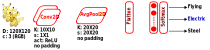
\includegraphics[width=0.8\textwidth]{../../img/workshop/CNN-pok-cls-en.pdf}
	\caption{Architecture of CNN-based Pokemon classification.}
	\label{fig:CNN-pok-cls}
\end{figure}

\subsection{Clustering-based classifier}

Design a model that takes the code generated by the previous auto-encoder and classifies the pokemon according to its type: 
\begin{itemize}
	\item You must use the previously trained encoder; i.e. the input must be an image and not the vector of its code. 
	Then the auto-encoder encodes the image using the \textbf{encode} method.
	\item The ranking model is an MLP (obviously!) that takes the encoder output as input and outputs the type of the pokemon.
	\item When training the workbook, you should not update the encoder; you must deactivate model training: \textbf{model.trainable = False}.
	\item Compare this model to that of classification (first section).
\end{itemize}

\section{Generation}

We want to design a model that generates new pokemons following these specifications: 
\begin{itemize}
	\item The code is a vector of 10 elements.
	\item Use CNNs to minimize the number of parameters.
	\item In addition to the latent variable, we must use a vector that represents the type, in order to learn how to generate a pokemon according to the type.
\end{itemize}

\subsection{Variational auto-encoder}

\begin{itemize}
	\item Similar to \textbf{ClusterCNNAE}, but the decoder has 3 vectors as input (see \ref{fig:gen-vae}).
\end{itemize}

\begin{figure}[htp]
	\centering
	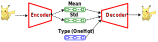
\includegraphics[width=0.48\textwidth]{../../img/workshop/VAE-en.pdf}
	\caption{Architecture of variational auto-encoder based Pokemon generator.}
	\label{fig:gen-vae}
\end{figure}

\subsection{GAN}

Generative Adversarial Network (GAN) is composed of two components: a generator and a discriminator (see figure \ref{fig:gen-gan}). 
The first one tries to generate images similar to the real ones.
The second tries to detect if an image is real or fake. 
So the generator's goal is to fool the discriminator so it classifies its generated images as real. 
On the other hand, the discriminator must improve so it can separate real images from those generated by the generator.
Given $ M $ real images, for each iteration:

\begin{itemize}
	\item Generate $ M $ images using the generator.
	\item Apply a forward pass on the discriminator by passing the $ 2M $ images.
	\item Calculate the classification error by considering the $ M $ real images as positive class (1) and the $ M $ generated images as negative class (0). 
	\item Update the discriminator's parameters using this error. This will ensure that the discriminator will learn to classify generated images as fake.
	\item Generate new $ M $ images using the generator.
	\item Apply a forward pass on the discriminator by passing only the $ M $ new generated images.
	\item Calculate the error by considering all these images as positive class (1); in this case they are considered as being real.
	\item This error will be used to update generator's parameters. In this case, when the discriminator could classify the images as fake, the error will be great and thus the generator will adapt so it can generate better images.
	\item Technically speaking, using tensorflow, we cannot inject an error directly into the backward pass without using the last activations (outputs).
	In this case, we will suppose that each output of the generator $S_i$ (where $S[32, 32, 3]$) is calculated using the error $J_D$ from the discriminator as follows:
	\[\frac{\partial J_D}{\partial S_i} = \frac{S_i * J_D}{\sum S_j}\]
	
\end{itemize}

\begin{figure}[htp]
	\centering
	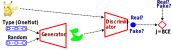
\includegraphics[width=0.48\textwidth]{../../img/workshop/GAN-en.pdf}
	\caption{Architecture of GAN based Pokemon generator.}
	\label{fig:gen-gan}
\end{figure}


\end{document}
